% !TeX root = ../thuthesis-example.tex

\chapter{部署平台设计}
一个完备的飞行部署平台应具备性能稳定、接口完善、易用性高等优点。目前市面上尚没有一种满足本研究算法部署需求的平台。本研究从硬件选型、装配再到部署系统的开发,设计了整个部署平台。本部署平台的开发参考了相关工作的开源硬件平台\cite{zhou2020ego}和控制系统\cite{Faessler18ral}。

\section{硬件平台搭建}

截止本报告撰写,为本研究设计的自主无人机已经迭代三个版本。如图\ref{}所示。最新版本自主无人机的基本参数如表\ref{tab_drone_param}所示。
% 详细的硬件平台选型及各部件基本参数以及三个版本无人机的功能改进如附录\ref{}所示。
\begin{table}
    \centering
    \begin{tabular}{cc}
    \hline
        项目名称 & 指标 \\ \hline
         轴距 & 250mm \\ 
        起飞重量 & ~ \\ 
        单轴推力 & ~ \\ 
        推重比 & ~ \\ 
         计算平台 & Nvidia Xavier NX $\times$ 2 \\ 
        CPU算力 & 6核心1.4GHz $\times$ 2 \\ 
        GPU算力 & 21TOPS $\times$ 2 \\ 
         飞行控制器 & CUAV V5+ \\ 
        飞行控制器频率 & 50$\sim$500Hz \\ \hline
    \end{tabular}
    \caption{无人机的基本参数}
    \label{tab_drone_param}
\end{table}


\section{部署系统}
本研究基于ROS开发了一套运行于机载计算机上的部署系统。部署系统的主要功能是收集传感器的输入、提供算法接口、为飞行器保证基本的飞行能力、以及与底层执行器(在本研究中是飞行控制器)通信。本研究开发的部署系统结构如图\ref{fig_deploy_framework}所示,每个框代表一个ROS节点。其中的AutoPilot节点是部署框架的核心节点。
\begin{figure}
    \centering
    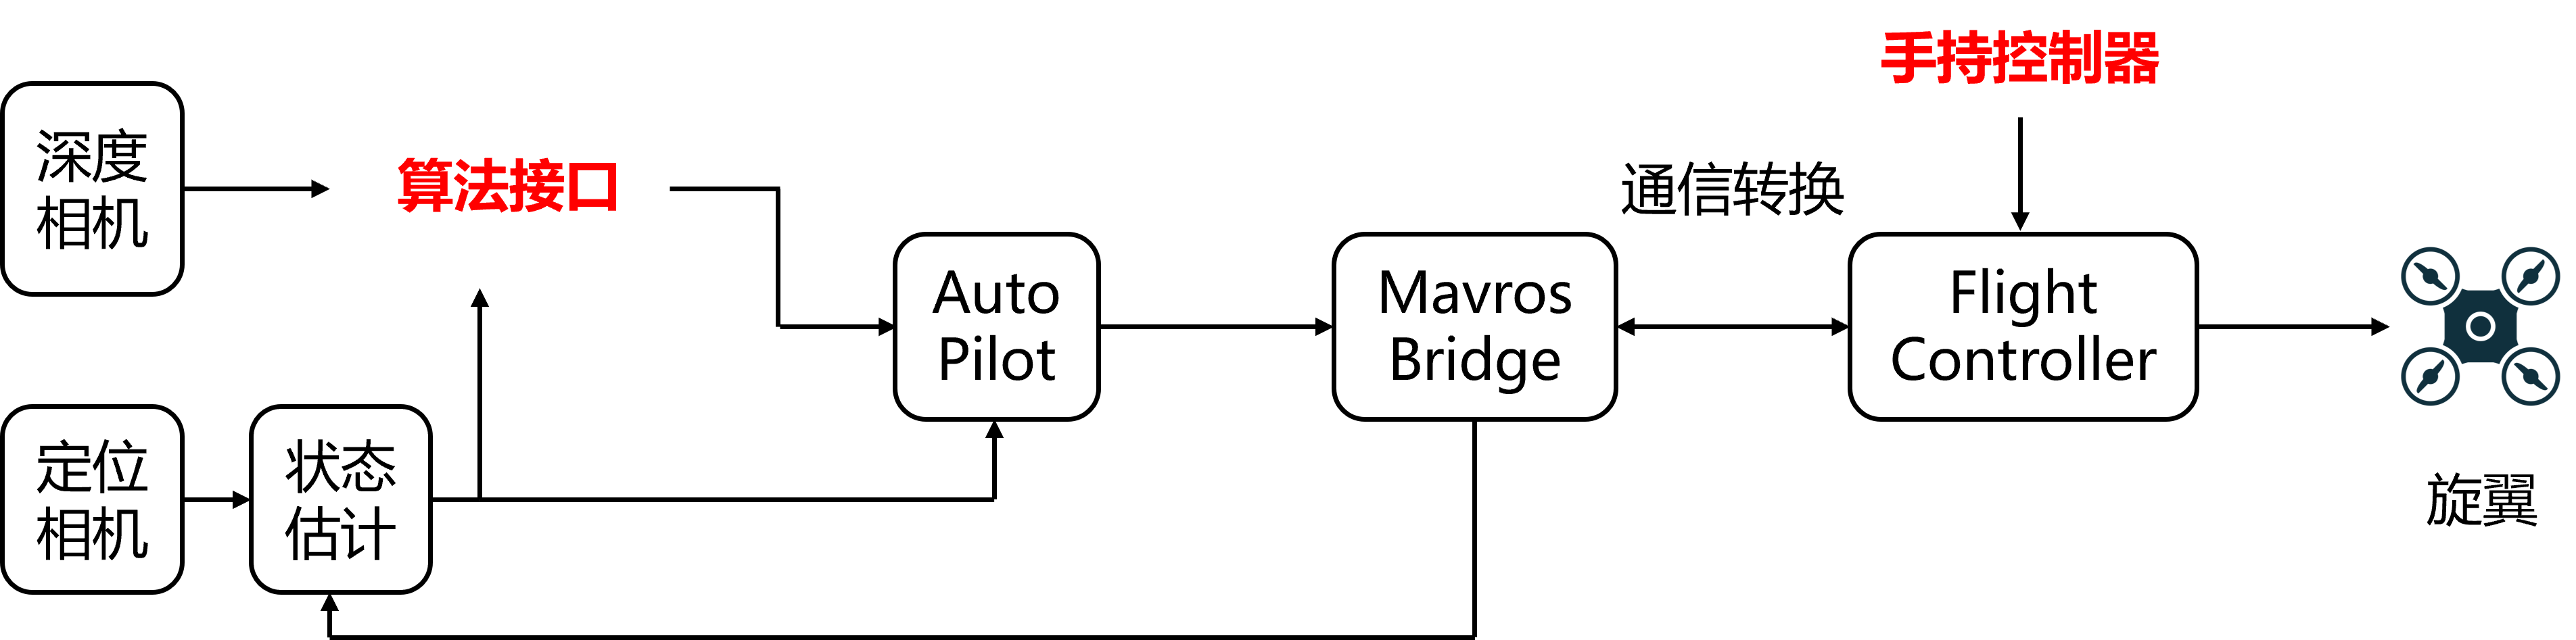
\includegraphics[width = 1\textwidth]{deploy_framework.png}
    \caption{部署系统结构图}
    \label{fig_deploy_framework}
\end{figure}

\subsection{系统输入}
系统的输入与表\ref{tab_input}所示一致。其中VIO的算法被嵌入式地集成到定位相机模块中,定位相机会直接输出飞行器的位置、姿态和速度信息。深度图的信息直接来源于深度相机模块。

为增强定位系统的稳定性,本研究同样使用飞行控制器携带的IMU读取位姿信息。部署系统与飞行控制器通过Mavros桥通信\cite{mavros2023},读取IMU信息并使用增强卡尔曼滤波\cite{kalman1960contributions}\cite{kalman1960new}\cite{kalman1961new}(extended Kalman filter, EKF)融合定位相机与IMU的信息,得到更可靠的飞行器位姿信息。

\subsection{算法接口}
本部署框架于Autopilot节点内集成了模型预测控制器\cite{Falanga2018}(Model predict control, MPC)和比例-积分-微分控制器(Proportion-integration-differentiation, PID)控制器。通过封装,两个控制器均可以接受五种不同的命令输入,并将他们转换为统一的输出。输出有两种模式可供选择。输入和输出命令的具体介绍如表\ref{tab_autopilot_input}和表\ref{tab_autopilot_output}所示。

\begin{table}
    \centering
    \begin{tabular}{ccl}
    \hline
        \textbf{输入名称} & \textbf{输入内容} & \textbf{输入描述} \\ \hline
        pos\_command & $(x,\ y,\ z)$ & 指定空间中一点,按照直线飞行至该位置。 \\ 
        velo\_command & $(v_x,\ v_y,\ v_z,\ \omega_{z})$ & 指定线速度和$z$向角速度,按照该速度飞行。 \\ 
        \multirow{3}*{ref\_command} & 一个轨迹点(Trajectory Point): & 指定轨迹点,使飞行器的状态与轨迹点尽 \\ 
        & $(x,\ y,\ z,\ \text{roll, pitch, yaw})$ & 可能接近。通常轨迹点与当前状态差别不 \\
        & 及其$1\sim3$阶时间导数 & 大,连续发送轨迹点以实现光滑控制。 \\
        traj\_command & 一串轨迹点 & 从初始位置连续飞行全部轨迹点 \\ 
        control\_command & 控制器输出的指令格式 & 控制器不工作 \\ \hline
    \end{tabular}
    \caption{集成控制器可选输入}
    \label{tab_autopilot_input}
\end{table}

\begin{table}
    \centering
    \begin{tabular}{ccl}
    \hline
        \textbf{输出模式} & \textbf{输出内容} & \textbf{输入描述} \\ \hline
        attitude & $(\text{thrust},\ \text{roll, pitch, yaw})$ & 飞行器的总推力和目标姿态 \\ 
        bodyrates & $(\text{thrust},\ \omega_x,\ \omega_y,\ \omega_z)$ & 即CTBR命令 \\ \hline
    \end{tabular}
    \caption{集成控制器可选输出}
    \label{tab_autopilot_output}
\end{table}

\subsection{状态切换}

AutoPilot节点同时负责无人机的飞行状态切换,其运行的是一个有限状态机(Finite State Machine, FSM)。FSM的状态转移图如图\ref{fig_fsm}所示。从图中可以看出该节点负责任务外的飞行模式,例如自动起降、自动悬停等。AutoPilot节点还为飞行系统带来了强大的鲁棒性,若飞行过程中感知或规划出现问题时,有限状态机会自动切换到悬停模式,保证飞行器的安全。该节点设置看门狗(WatchDog)线程,飞行过程中控制器出现问题时,节点会自动发出告警并切换至手动飞行模式。此外该节点还负责读取飞行控制器的反馈,例如电机温度、电池电压、电流等参数,根据参数随时改变规划器和控制器的参数,实现更高精度的飞行。

\begin{figure}
    \centering
    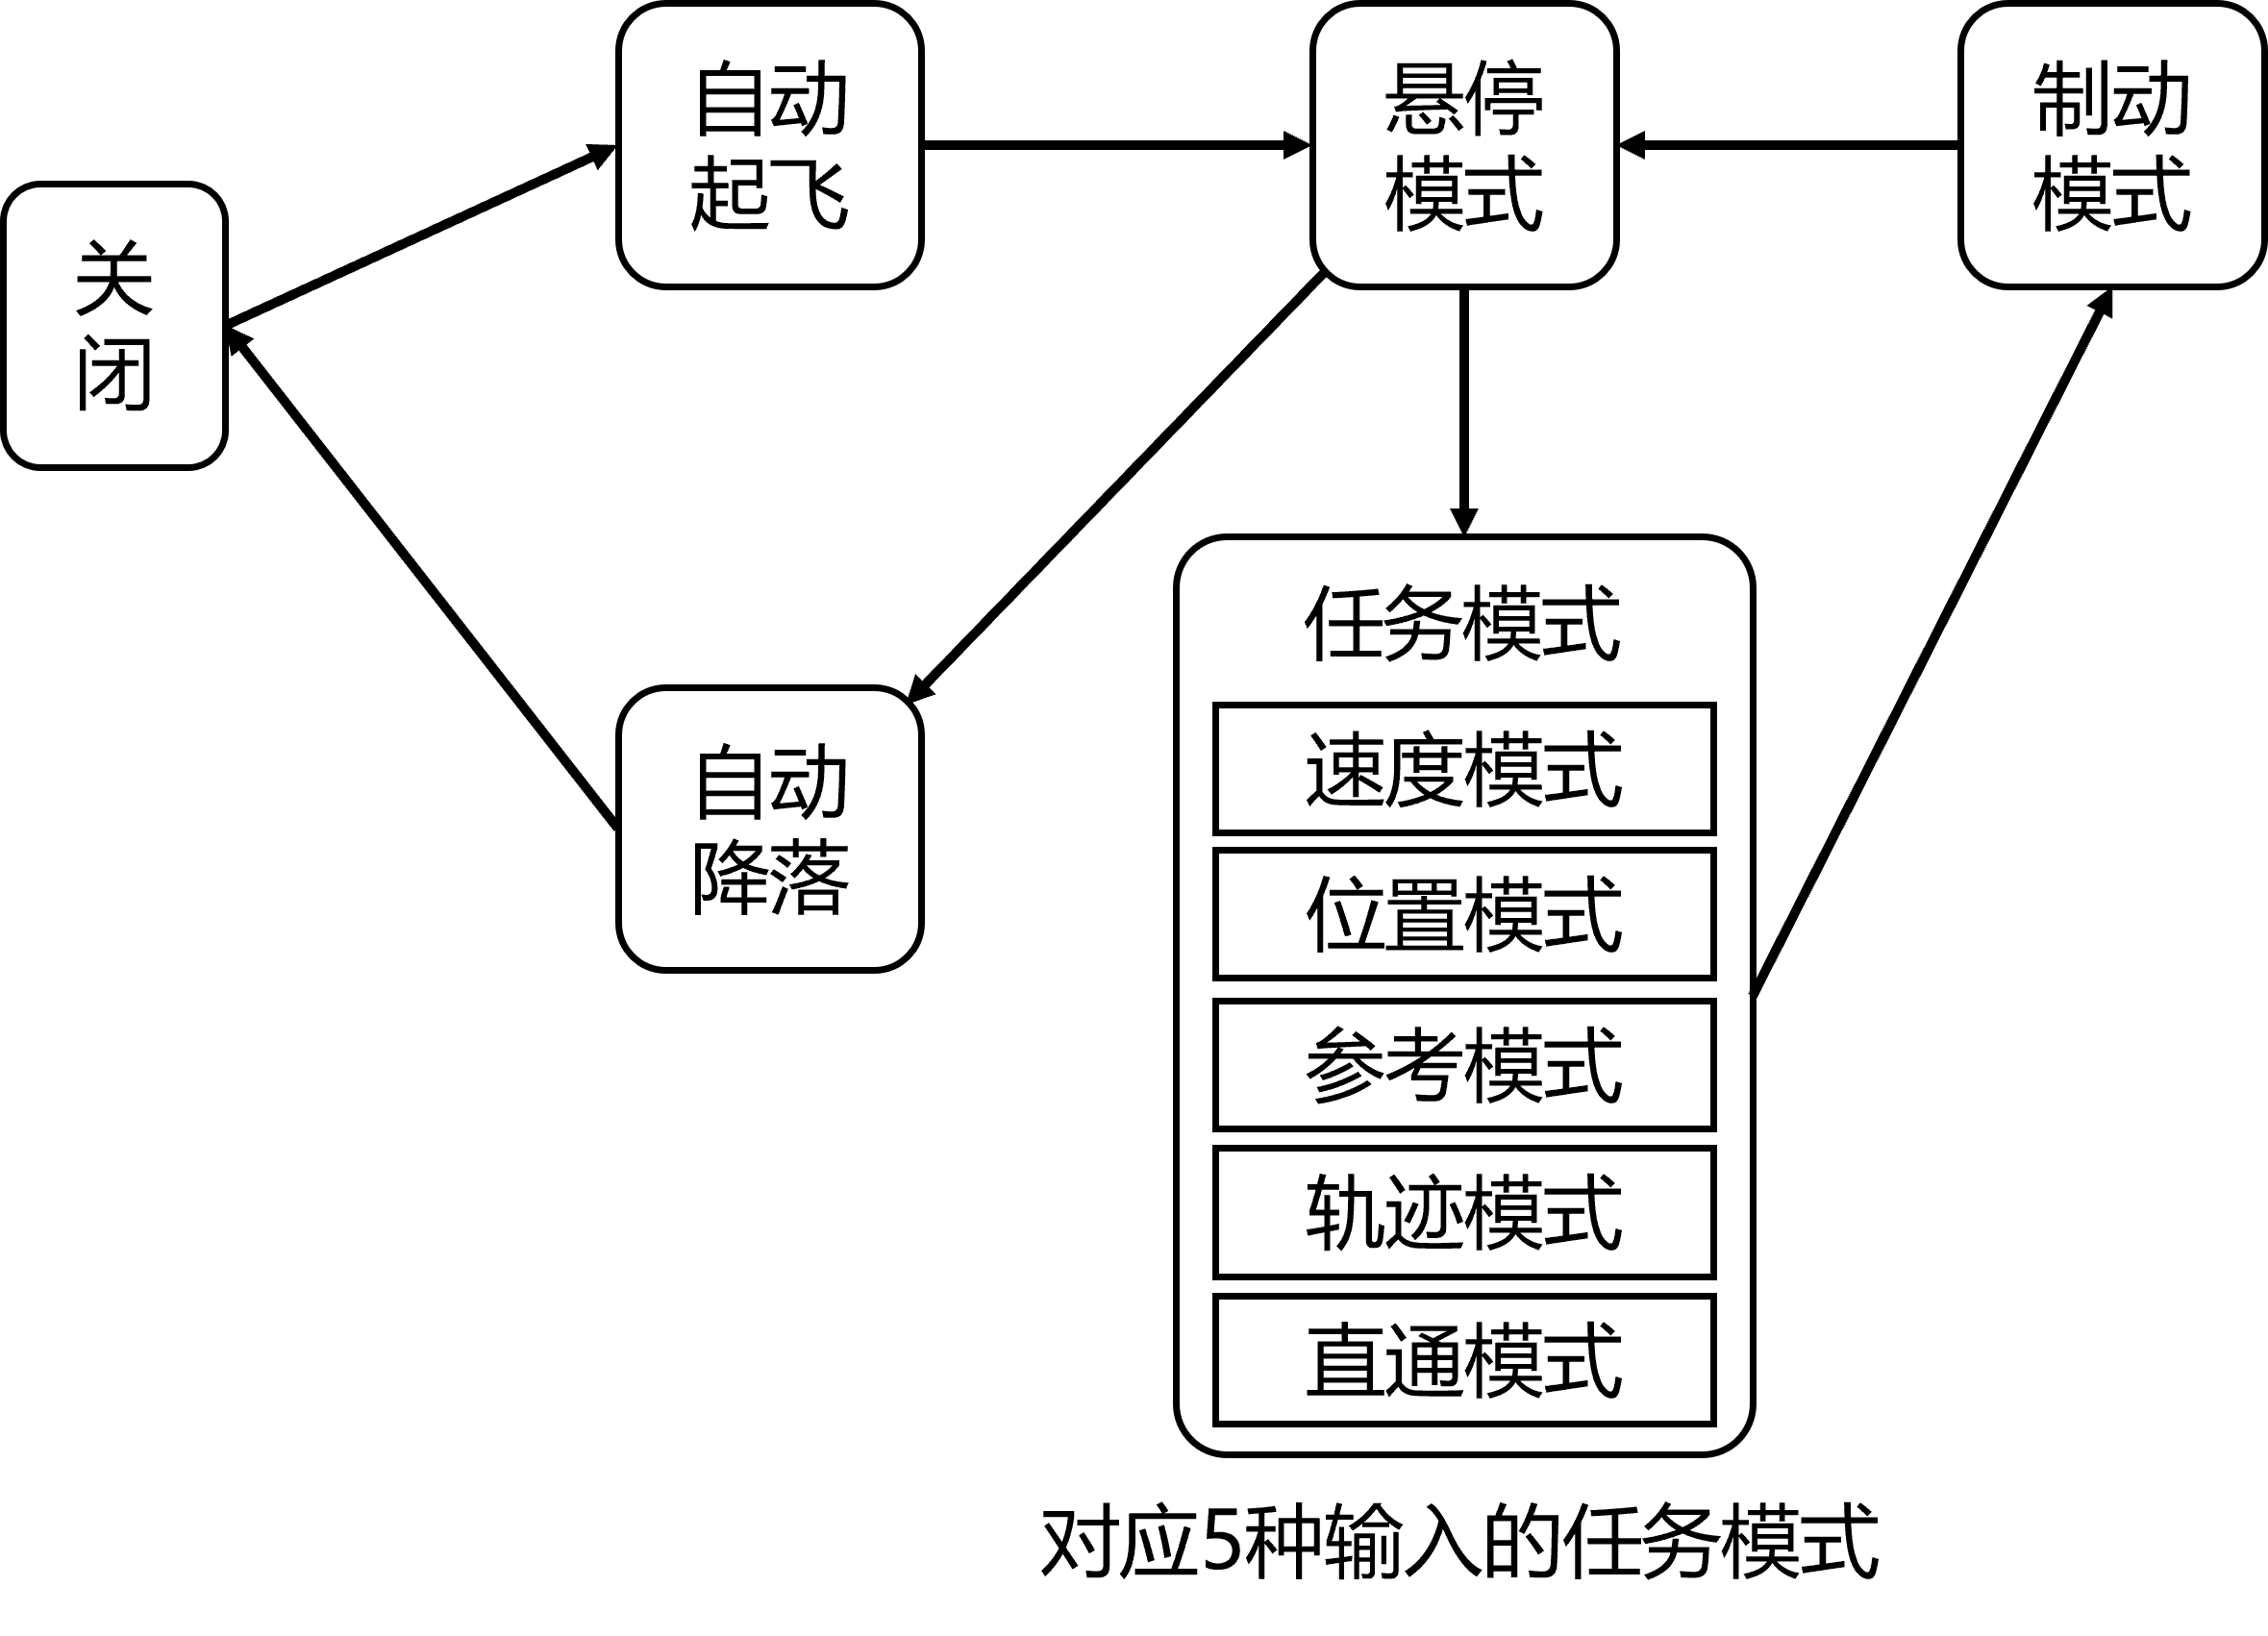
\includegraphics[width = 0.7\textwidth]{fsm.png}
    \caption{状态转移图}
    \label{fig_fsm}
\end{figure}

\subsection{部署系统的基本性能}
部署系统的性能受硬件选型、驱动、软件设计等多方面因素制约。经测试将本部署平台的基础性能制成表\ref{tab_deploy}。

\begin{table}
    \centering
    \begin{tabular}{ccc}
    \hline
         名称 & 指标 & 备注 \\ \hline
        深度图尺寸 & $640\times 320$ & ~ \\ 
        深度图精度 & $<2\%$ & 在$2m$位置处 \\ 
        深度图频率 & $30Hz$ & ~ \\ 
        视觉里程计频率 & $200Hz$ & 使用EKF融合IMU输出后的频率 \\ 
        视觉里程计精度 & $<0.02m$ & 室内任务,时间约30s,轨迹长度约$20m$ \\ 
        控制器频率 & $200Hz$ & ~ \\ 
        修正参数频率 & $1Hz$ & ~ \\ 
        最大飞行速度 & $7m/s$ & ~ \\ 
        最大飞行加速度 & $5m/s^2$ & ~ \\ 
        轨迹跟踪精度 & $<0.1m$ & 室内场景飞行8字轨迹,飞行速度$3m/s$,最小曲率半径$1.5m$ \\ \hline
    \end{tabular}
    \caption{部署平台基础性能表}
    \label{tab_deploy}
\end{table}

特别地,本部署平台与仿真平台使用了同样的算法接口,因此本部署平台支持沙盒操作,即同时启动仿真平台和部署平台,利用Rviz可视化工具实时可视化部署平台的状态并进行操作。图\ref{fig_flight}和\ref{fig_sandbox}是沙盒操作的示意图。图\ref{fig_flight}是无人机在执行室内飞行任务的照片,图\ref{fig_sandbox}是同一时刻实时可视化的飞行器状态、环境建图和正在执行的8字形轨迹。
\begin{figure}
    \centering
    \includegraphics[width = 1\textwidth]{flight.png}
    \caption{室内飞行任务}
    \label{fig_flight}
\end{figure}
\begin{figure}
    \centering
    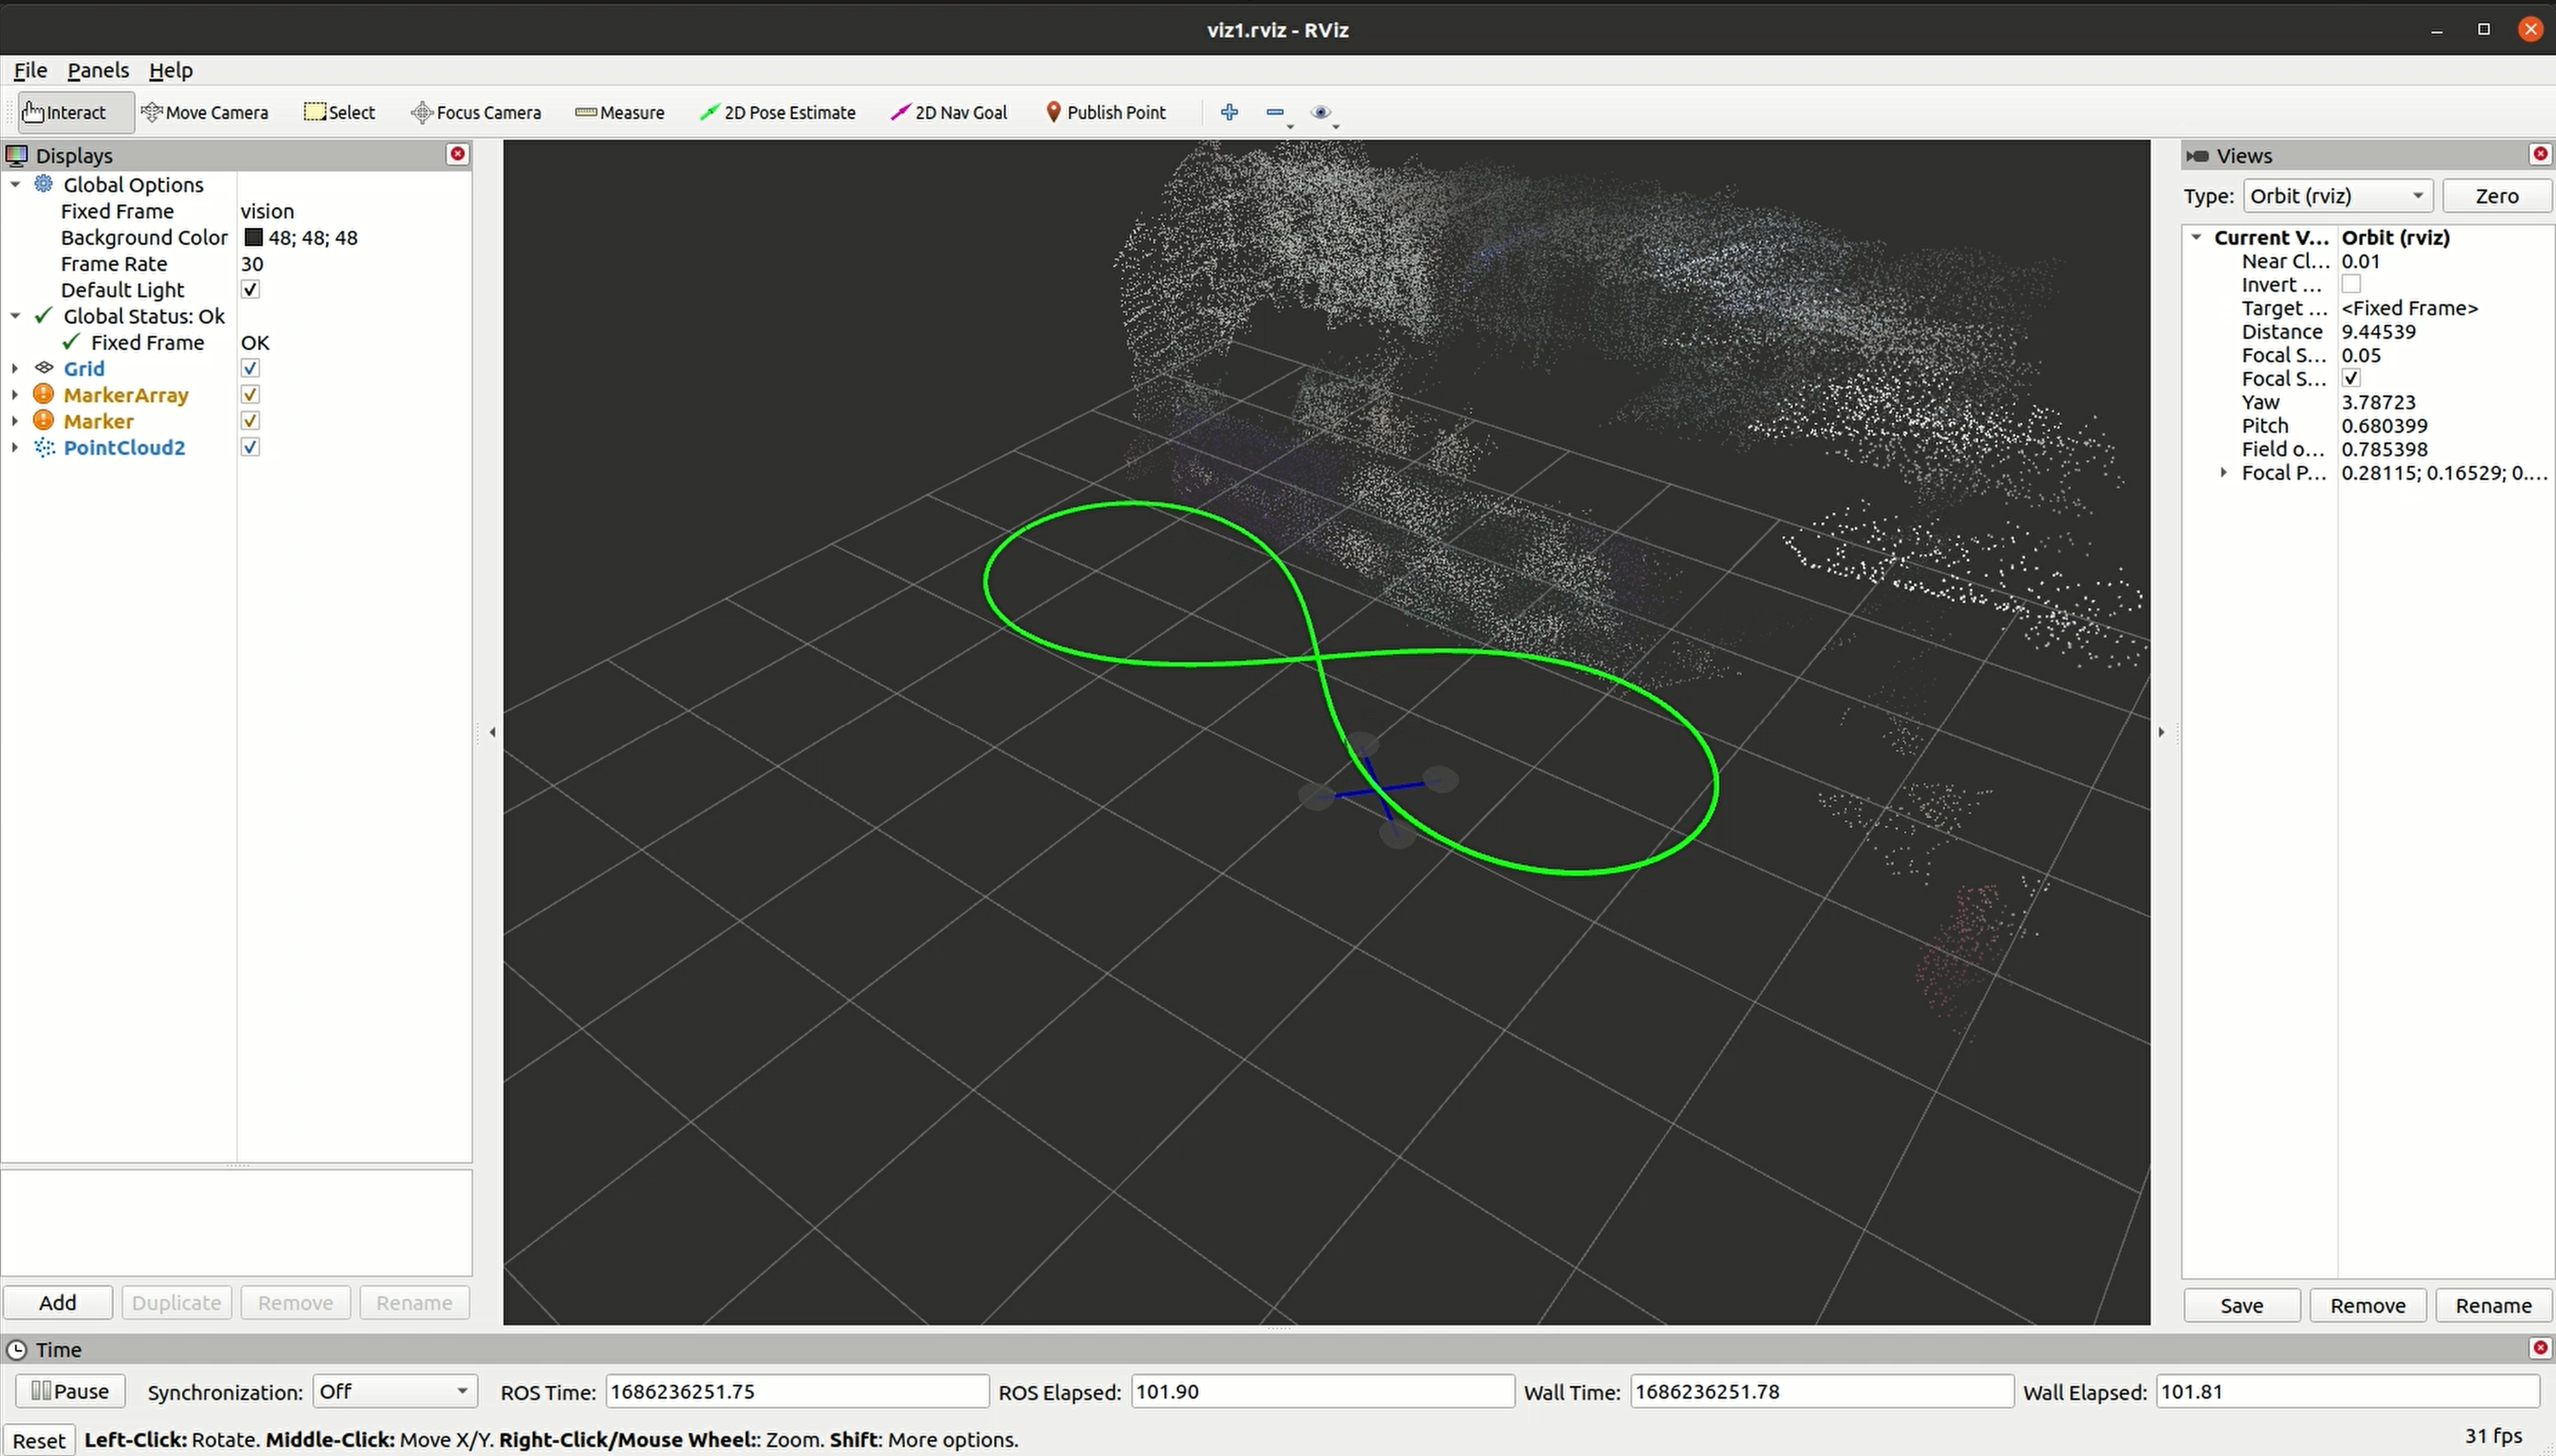
\includegraphics[width = 1\textwidth]{sandbox.png}
    \caption{沙盒操作示意图}
    \label{fig_sandbox}
\end{figure}

\subsection{本章小结}

本章从硬件搭建和部署系统开发两个层面介绍了本研究的部署平台。该部署平台是本研究的另一项重要工作。本部署平台具有完善的自主感知和机载计算能力,且拥有敏捷飞行的能力。而配套的部署系统为无人机提供了可靠的控制、通信、基础飞行和异常处理的能力,接口丰富、运行稳定。在室内和场景不特别空旷的室外,该系统表现出良好的飞行性能。将训练好的算法部署到该系统上的飞行表现将在第\ref{result}章中介绍

%此处应包含部署系统的基础能力测试

% 模板支持 BibTeX 和 BibLaTeX 两种方式处理参考文献。
% 下文主要介绍 BibTeX 配合 \pkg{natbib} 宏包的主要使用方法。


% \section{顺序编码制}

% 在顺序编码制下,默认的 \cs{cite} 命令同 \cs{citep} 一样,序号置于方括号中,
% 引文页码会放在括号外。
% 统一处引用的连续序号会自动用短横线连接。

% \thusetup{
%   cite-style = super,
% }
% \noindent
% \begin{tabular}{l@{\quad$\Rightarrow$\quad}l}
%   \verb|\cite{zhangkun1994}|               & \cite{zhangkun1994}               \\
%   \verb|\citet{zhangkun1994}|              & \citet{zhangkun1994}              \\
%   \verb|\citep{zhangkun1994}|              & \citep{zhangkun1994}              \\
%   \verb|\cite[42]{zhangkun1994}|           & \cite[42]{zhangkun1994}           \\
%   \verb|\cite{zhangkun1994,zhukezhen1973}| & \cite{zhangkun1994,zhukezhen1973} \\
% \end{tabular}


% 也可以取消上标格式,将数字序号作为文字的一部分。
% 建议全文统一使用相同的格式。

% \thusetup{
%   cite-style = inline,
% }
% \noindent
% \begin{tabular}{l@{\quad$\Rightarrow$\quad}l}
%   \verb|\cite{zhangkun1994}|               & \cite{zhangkun1994}               \\
%   \verb|\citet{zhangkun1994}|              & \citet{zhangkun1994}              \\
%   \verb|\citep{zhangkun1994}|              & \citep{zhangkun1994}              \\
%   \verb|\cite[42]{zhangkun1994}|           & \cite[42]{zhangkun1994}           \\
%   \verb|\cite{zhangkun1994,zhukezhen1973}| & \cite{zhangkun1994,zhukezhen1973} \\
% \end{tabular}



% \section{著者-出版年制}

% 著者-出版年制下的 \cs{cite} 跟 \cs{citet} 一样。

% \thusetup{
%   cite-style = author-year,
% }
% \noindent
% \begin{tabular}{@{}l@{$\Rightarrow$}l@{}}
%   \verb|\cite{zhangkun1994}|                & \cite{zhangkun1994}                \\
%   \verb|\citet{zhangkun1994}|               & \citet{zhangkun1994}               \\
%   \verb|\citep{zhangkun1994}|               & \citep{zhangkun1994}               \\
%   \verb|\cite[42]{zhangkun1994}|            & \cite[42]{zhangkun1994}            \\
%   \verb|\citep{zhangkun1994,zhukezhen1973}| & \citep{zhangkun1994,zhukezhen1973} \\
% \end{tabular}

% \vskip 2ex
% \thusetup{
%   cite-style = super,
% }
% 注意,引文参考文献的每条都要在正文中标注
% \cite{zhangkun1994,zhukezhen1973,dupont1974bone,zhengkaiqing1987,%
%   jiangxizhou1980,jianduju1994,merkt1995rotational,mellinger1996laser,%
%   bixon1996dynamics,mahui1995,carlson1981two,taylor1983scanning,%
%   taylor1981study,shimizu1983laser,atkinson1982experimental,%
%   kusch1975perturbations,guangxi1993,huosini1989guwu,wangfuzhi1865songlun,%
%   zhaoyaodong1998xinshidai,biaozhunhua2002tushu,chubanzhuanye2004,%
%   who1970factors,peebles2001probability,baishunong1998zhiwu,%
%   weinstein1974pathogenic,hanjiren1985lun,dizhi1936dizhi,%
%   tushuguan1957tushuguanxue,aaas1883science,fugang2000fengsha,%
%   xiaoyu2001chubanye,oclc2000about,scitor2000project%
% }。
